\documentclass[a4paper,12pt]{article} 

% packages and main settings
\usepackage[left=3cm, right=2cm, top=2cm, bottom=2cm]{geometry}
\usepackage[english]{babel}    
\usepackage[utf8]{inputenc}  
\usepackage[T1]{fontenc}        
\usepackage{lmodern}            
\usepackage{microtype}          
\usepackage{amsmath}
\usepackage{amsfonts, amsthm, amssymb, graphicx, booktabs}
\usepackage{bm} %bold epsilon
\usepackage{newclude}   
\usepackage{placeins}  %surpresses floating tables
\usepackage[labelfont=bf]{caption} %Figure etc steht dann in small caps 
\usepackage[labelsep=period]{caption} % dot after figure, table caption.
\usepackage[flushleft]{threeparttable} % for notes below table
\usepackage{multirow} % for table cell merge along rows
\usepackage{graphicx} % to adjust tablesize to textwidth
\usepackage{caption}  % for centered captions
\usepackage{float} % to set of autopositioning of tables
\usepackage[bottom,hang,flushmargin]{footmisc} % forces footnotes to the bottom
\usepackage{setspace}           % Fuer 1.5 fachen Zeilenabstand  
\onehalfspacing % 1.5 cm Zeilenabstand
%Bibtex
\usepackage[round,sort&compress]{natbib}

\bibliographystyle{chicago} % chicago bib style like in AER
\usepackage[hidelinks]{hyperref} % fuer links und verweise. Cleverref ist eigentlich besser. 


% Create header. The header must be surpressed for 
% every first page per section and a solution
% for the Appendix is used in the respective subfile.
\usepackage{fancyhdr}
\pagestyle{fancy}
\fancyhf{}
\chead{\nouppercase{\textit{\leftmark}}}
\cfoot{\thepage}
\renewcommand{\headrulewidth}{0pt} % no vertical line

%\usepackage{lipsum}  % check if formats work

\usepackage{afterpage} %clearpage w/o pagebreak for "header bug"

% Expectation symbol
\DeclareMathOperator*{\E}{\mathbb{E}}

% thin space, limits underneath in displays
% for strike through
\DeclareMathOperator*{\argmax}{argmax}
\newcommand*{\defeq}{\stackrel{\text{def}}{=}}
\usepackage[normalem]{ulem}
% try to use strikeout in section headers and others
\DeclareRobustCommand{\hsout}[1]{\texorpdfstring{\sout{#1}}{#1}}

% for gray table row color
\usepackage[table]{xcolor}

% decimal dot alignment in table columns
\usepackage{siunitx}

% for footnotes in table
\usepackage[flushleft]{threeparttable}

% for underbar
\newcommand{\ubar}[1]{\text{\b{$#1$}}}

\usepackage{tikz}

% Setup for urls
\usepackage{url}

\defcitealias{Respy-Stenzel.2019}{\textit{respy}}
\defcitealias{Gabler.2019}{\textit{estimagic}}
\defcitealias{Stenzel.2020}{\textit{Master's Thesis Replication Repository}}
\defcitealias{NLSY79}{NLSY79}


\usepackage{tikz}
\begin{document}

\newpage % delete after section is complete

\section{Results}

The section is divided in two parts. First, I present the results of the uncertainty analysis for an overview of the general variation in QoI $Y$. Thereafter, I present the results of the qualitative GSA. The aim is to draw inferences about the contribution of an individual input $X_i$ and its uncertainty on the uncertainty in QoI $Y$ to a degree that allows the identification of non-influential parameters.

\subsection{Uncertainty Analysis}
The following results are obtained by evaluating the occupational choice model at each parameter vector from a random sample. This sample is drawn from the estimated joint distribution. The number of draws is $10,000$. A reasonable level of convergence has already been achieved after about 800 evaluation.\footnote{See the respective notebook in the \citetalias{Stenzel.2020}.}


Figure \ref{fig:uq_paths} incorporates the input uncertainty in the shares of life-time occupation decisions that we have previously seen in Figure \ref{fig:paths}. It depicts the mean and the intervals for $99\%$ of the shares' probability distribution. We can see that the input uncertainty has an effect on the decisions for white- and blue-collar occupation but almost none on the decision for occupation in the education and home sector. This suggests that individuals mainly tend to change between occupation in blue- and white-collar occupation given the distribution of input parameters. Yet, the uncertainty in the shares for both labour sectors is not strikingly large. There is also no visible difference in the uncertainties between both scenarios.
\begin{figure}[H]
	\caption{Comparison of shares of occupation decision over time between scenarios including 99$\%$ confidence intervals}
	\centering
	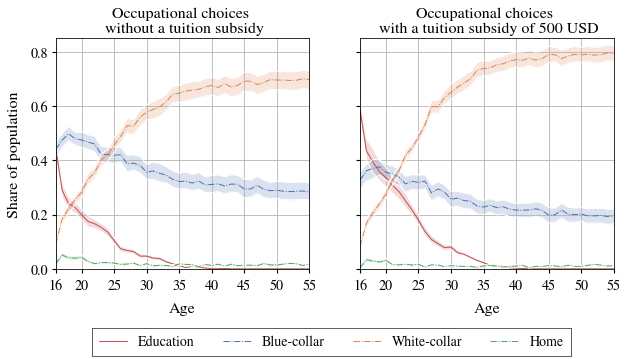
\includegraphics[scale=0.75]{../../../scrypy/figures/cone_plot_choice_shares}
	\label{fig:uq_paths}
\end{figure}

\noindent
Figure \ref{fig:dist} shows the probability distribution for QoI $Y$. The colorised bars depict the realisations within one and two and outside of two standard deviations, $\sigma_Y$, from sample mean $\overline{Y}$.  The distribution is minimally skewed to the left but can be considered as almost normal. This leads to the first conclusion for a potential quantitative GSA. That is, variance-based measures like Sobol' indices can be used because the variance is a good summary measure for normally distributed random variables.

Standard deviation $\sigma_Y$ equals 0.1 and variance $\sigma_Y^2$ equals 0.01. The final goal of a quantitative GSA is to compute the share that input parameter $X_i$ and its variation contribute to $\sigma_Y$ or $\sigma_Y^2$. We can expect that reasonable measures for the contribution of $X_i$ are not completely detached from the measures for the total variation in $Y$ if they are on the same scale. As we have seen earlier, for a linear function without interactions and correlations, we would even expect that the contribution of $X_i$ are smaller than the measure for the variation in $Y$.

The next section computes measures for these contributions.\footnote{For QoI $Y$, it is not necessary to compute the probabilities for specific regions in the probability space of $Y$. The reasons is that, for example in contrary to models for nuclear power plants, there are no regions that are particularly critical.}
\begin{figure}[H]
	\caption{Probability distribution of quantity of interest $q$}
	\centering
	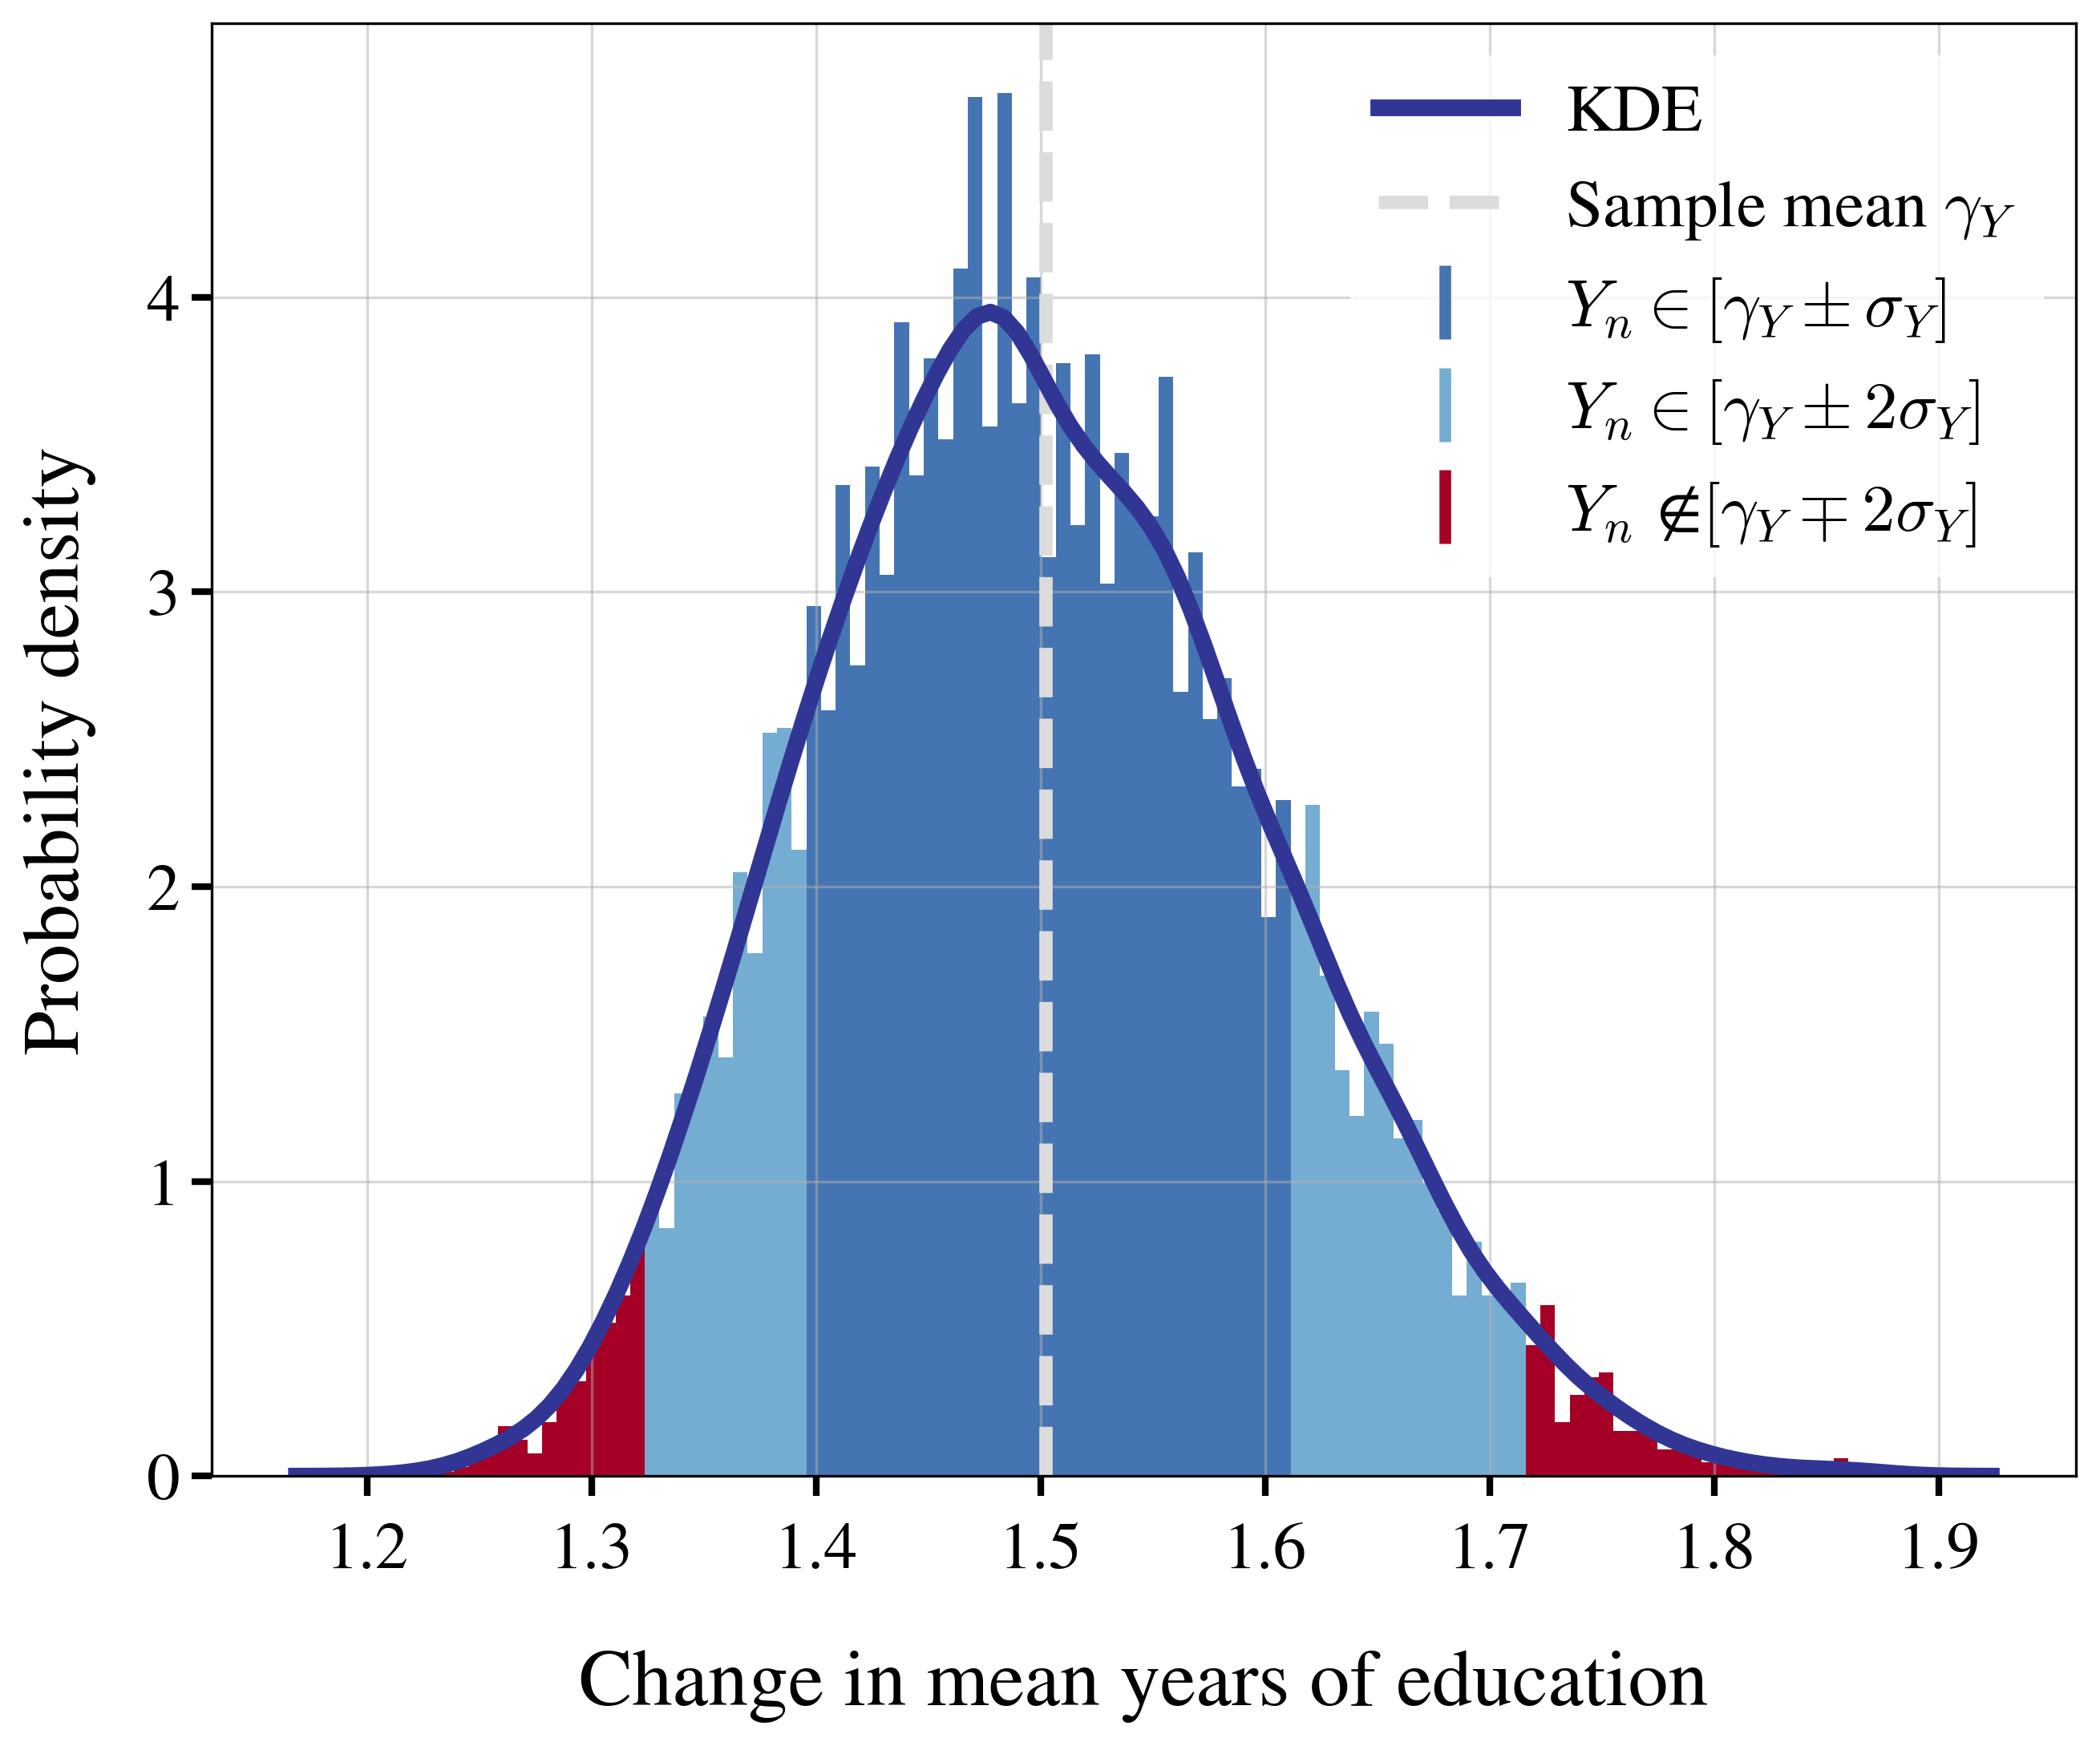
\includegraphics[scale=0.5]{../../../scrypy/figures/distplot}
	\label{fig:dist}
\end{figure}


\newpage
\subsection{Experiment \cite{ge2017extending}}
\newpage
\setlength{\tabcolsep}{22pt} %from 6
\begin{table}[H] 
	\centering
	\begin{threeparttable}
		\caption[Model Parametrization]{EE-based measures by \cite{ge2017extending} for 100 trajectories}
		\label{tab:gm17measures_traj}
		\renewcommand{\arraystretch}{1.2}%
		\begin{tabular}{cS[table-format=3.2]S[table-format=3.2]@{\hskip 0.7in}|@{\hskip 0.5in}S[table-format=3.2]S[table-format=3.2]}
			
			{Parameter}     & {$\mu^{*,full}_T$}   & {$\mu^{*,ind}_T$} & {$\sigma^{*,full}_T$} & {$\sigma^{*,ind}_T$}\\ \midrule
			\textit{General} \\
			$\delta$ & 53.40   & 0.00 & 69.23 & 0.09   \\    \midrule
			\textit{Blue-collar}\\    
			$\beta^b$ & 3.55   & 0.05            & 4.38 & 0.07    \\
			$\beta_e^b$ & 39.84  &    0.05        & 49.69  & 0.07    \\
			$\beta^b_b$ & 77.21  & 0.05            & 90.23  & 0.07    \\
			$\beta^b_{bb}$ & 2616.50 & 0.05           & 3357.92  & 0.06     \\
			$\beta^b_w$ & 94.74    & 0.05             & 113.49  &  0.06  \\
			$\beta^b_{ww}$ & 1136.58    & 0.03          & 1405.94 &  0.04    \\ \midrule
			\textit{White-collar}\\
			$\beta^w$ & 5.07   & 0.05            & 6.42 &  0.06   \\
			$\beta^w_e$ & 90.25   & 0.07          & 111.50 &  0.08    \\
			$\beta^w_w$ & 82.88  & 0.05            & 103.66 &  0.07   \\
			$\beta^w_{ww}$ & 2444.13  & 0.06           & 3044.69 & 0.07   \\
			$\beta^w_b$ & 452.91 & 0.07           & 490.31 &  0.09   \\
			$\beta^w_{bb}$ & 4317.58 & 0.05         & 4851.54 &  0.06   \\ \midrule
			\textit{Education} \\
			$\beta^e$     & 0.00    & 0.09             & 0.00&  0.10   \\
			$\beta_{he}^e$     & 0.00    & 0.11              & 0.00  & 0.13    \\
			$\beta_{re}^e$     & 0.00  & 0.04               & 0.000  &   0.09  \\ \midrule
			\textit{Home} \\
			$\beta^h$    & 0.00  & 0.04                 & 0.00  & 0.05     \\ \midrule
			\multicolumn{4}{l}{\textit{Lower Triangular Cholesky Matrix}} \\
			$c_{1}$      & 27.94    & 0.07             & 33.72 &  0.08   \\
			$c_{2}$      & 31.89   & 0.05             & 38.58 & 0.06   \\
			$c_{3}$      & 0.00   & 0.06             & 0.00 & 0.07    \\
			$c_{4}$      & 0.00    & 0.04              & 0.00 & 0.09    \\
			$c_{1,2}$     & 12.41   & 0.06            & 14.33 &  0.08  \\
			$c_{1,3}$      & 0.00   & 0.09              & 0.00 &  0.10   \\
			$c_{2,3}$      & 0.00    & 0.05             &  0.00 &   0.06 \\
			$c_{1,4}$      & 0.00    & 0.04            &   0.00 &  0.05 \\
			$c_{2,4}$      & 0.00    & 0.03           & 0.00  &  0.03  \\
			$c_{3,4}$      & 0.00   & 0.04                & 0.00  &  0.05   \\ \bottomrule
		\end{tabular}
	\end{threeparttable}
\end{table}
\newpage



\subsection{Qualitative Sensitivity Analysis}
\newpage
\setlength{\tabcolsep}{22pt} %from 6
\begin{table}[H] 
	\centering
	\begin{threeparttable}
		\caption[Model Parametrization]{Mean absolute correlated and uncorrelated elementary effects\\ (based on 100 subsamples in trajectory and radial design)}
		\label{tab:params}
		\renewcommand{\arraystretch}{1.2}%
		\begin{tabular}{cS[table-format=3.2]S[table-format=3.2]@{\hskip 0.7in}|@{\hskip 0.5in}S[table-format=3.2]S[table-format=3.2]}

			{Parameter}     & {$\mu^{*,c}_T$}   & {$\mu^{*,c}_R$} & {$\mu^{*,u}_T$} & {$\mu^{*,u}_R$}\\ \midrule
			\textit{General} \\
			$\delta$ & 17   & 23 & 476 & 415   \\    \midrule
			\textit{Blue-collar}\\    
			$\beta^b$ & 1   & 3            & 43 & 88    \\
			$\beta_e^b$ & 11  &    14        & 406  & 443    \\
			$\beta^b_b$ & 25  & 51            & 688  & 1169    \\
			$\beta^b_{bb}$ & 871 & 934           & 15540  & 17860     \\
			$\beta^b_w$ & 29    & 48             & 73  &  143  \\
			$\beta^b_{ww}$ & 389    & 460           & 869 &  1183    \\ \midrule
			\textit{White-collar}\\
			$\beta^w$ & 1   & 3            & 50 &  117   \\
			$\beta^w_e$ & 26   & 28          & 943 &  852    \\
			$\beta^w_w$ & 24  & 47            & 718 &  1521   \\
			$\beta^w_{ww}$ & 933  & 997           & 12257 & 18069   \\
			$\beta^w_b$ & 131 & 127           & 309 &  356   \\
			$\beta^w_{bb}$ & 120 & 1352         & 2088 &  2477   \\ \midrule
			\textit{Education} \\
			$\beta^e$     & 0.0008    & 0.0002              & 0.001&  0.003   \\
			$\beta_{he}^e$     & 0.0001    & 0.0002              & 0.001  & 0.001    \\
			$\beta_{re}^e$     & 0.0003   & 0.0002               & 0.0003  &   0.0006  \\ \midrule
			\textit{Home} \\
			$\beta^h$    & 0.0003  & 0.0003                 & 0.00002  & 0.00002     \\ \midrule
			\multicolumn{4}{l}{\textit{Lower Triangular Cholesky Matrix}} \\
			$c_{1}$      & 8    & 16             & 18 &  37   \\
			$c_{2}$      & 8   & 11             & 22 & 24   \\
			$c_{3}$      & 0.0004   & 0.0004             & 0.0004 & 0.0007    \\
			$c_{4}$      & 0.0004    & 0.00008              & 0.0002 & 0.0003    \\
			$c_{1,2}$     & 4   & 4            & 10 &  10  \\
			$c_{1,3}$      & 0.0005   & 0.0006              & 0.0006 &  0.0005   \\
			$c_{2,3}$      & 0.0003    & 0.0005             &  0.0006 &   0.001 \\
			$c_{1,4}$      & 0.00004    & 0.00005            &   0.0004 &  0.0005 \\
			$c_{2,4}$      & 0.0001    & 0.0002           & 0.0001  &  0.0002  \\
			$c_{3,4}$      & 0.0001   & 0.0001                & 0.00008  &  0.0001   \\ \bottomrule
		\end{tabular}
	\end{threeparttable}
\end{table}
\newpage
\begin{figure}[H]
	\caption{Sigma-normalized mean absolute Elementary Effects for trajectory design}
	\centering
	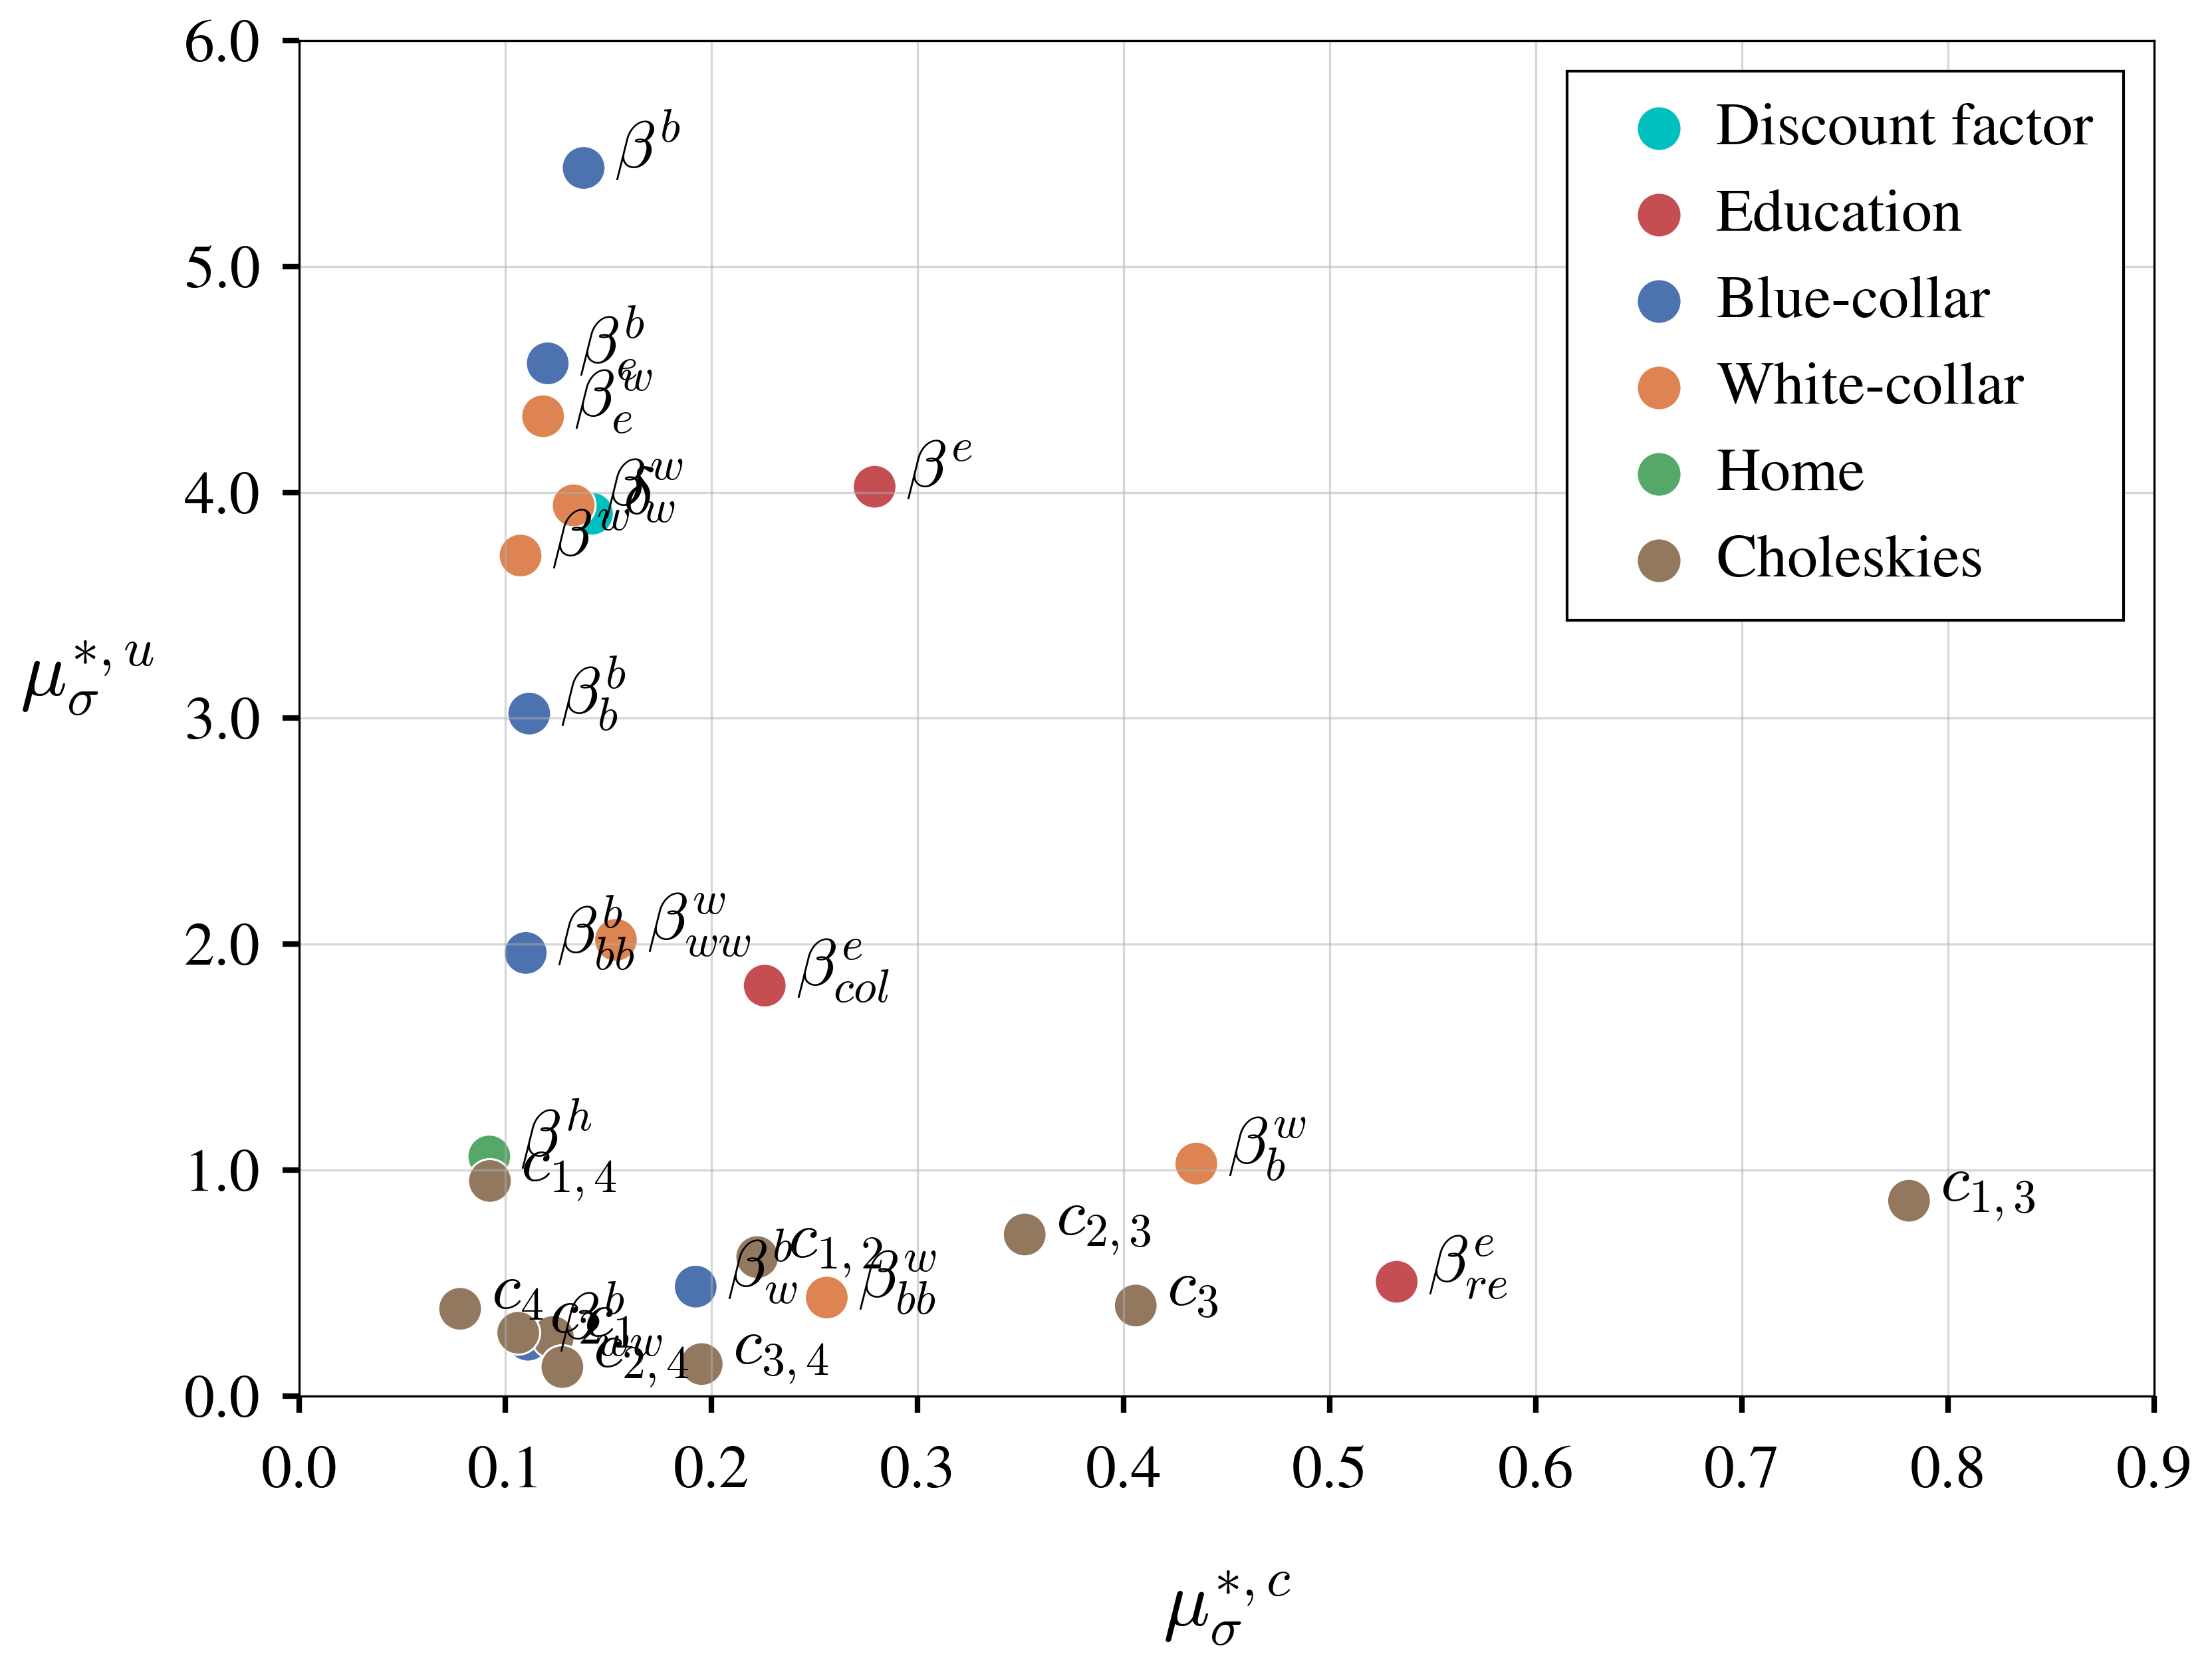
\includegraphics[scale=0.52]{../../../scrypy/figures/scatter_traj}
	\label{fig:traj}
\end{figure}

\begin{figure}[H]
	\caption{Sigma-normalized mean absolute Elementary Effects for radial design}
	\centering
	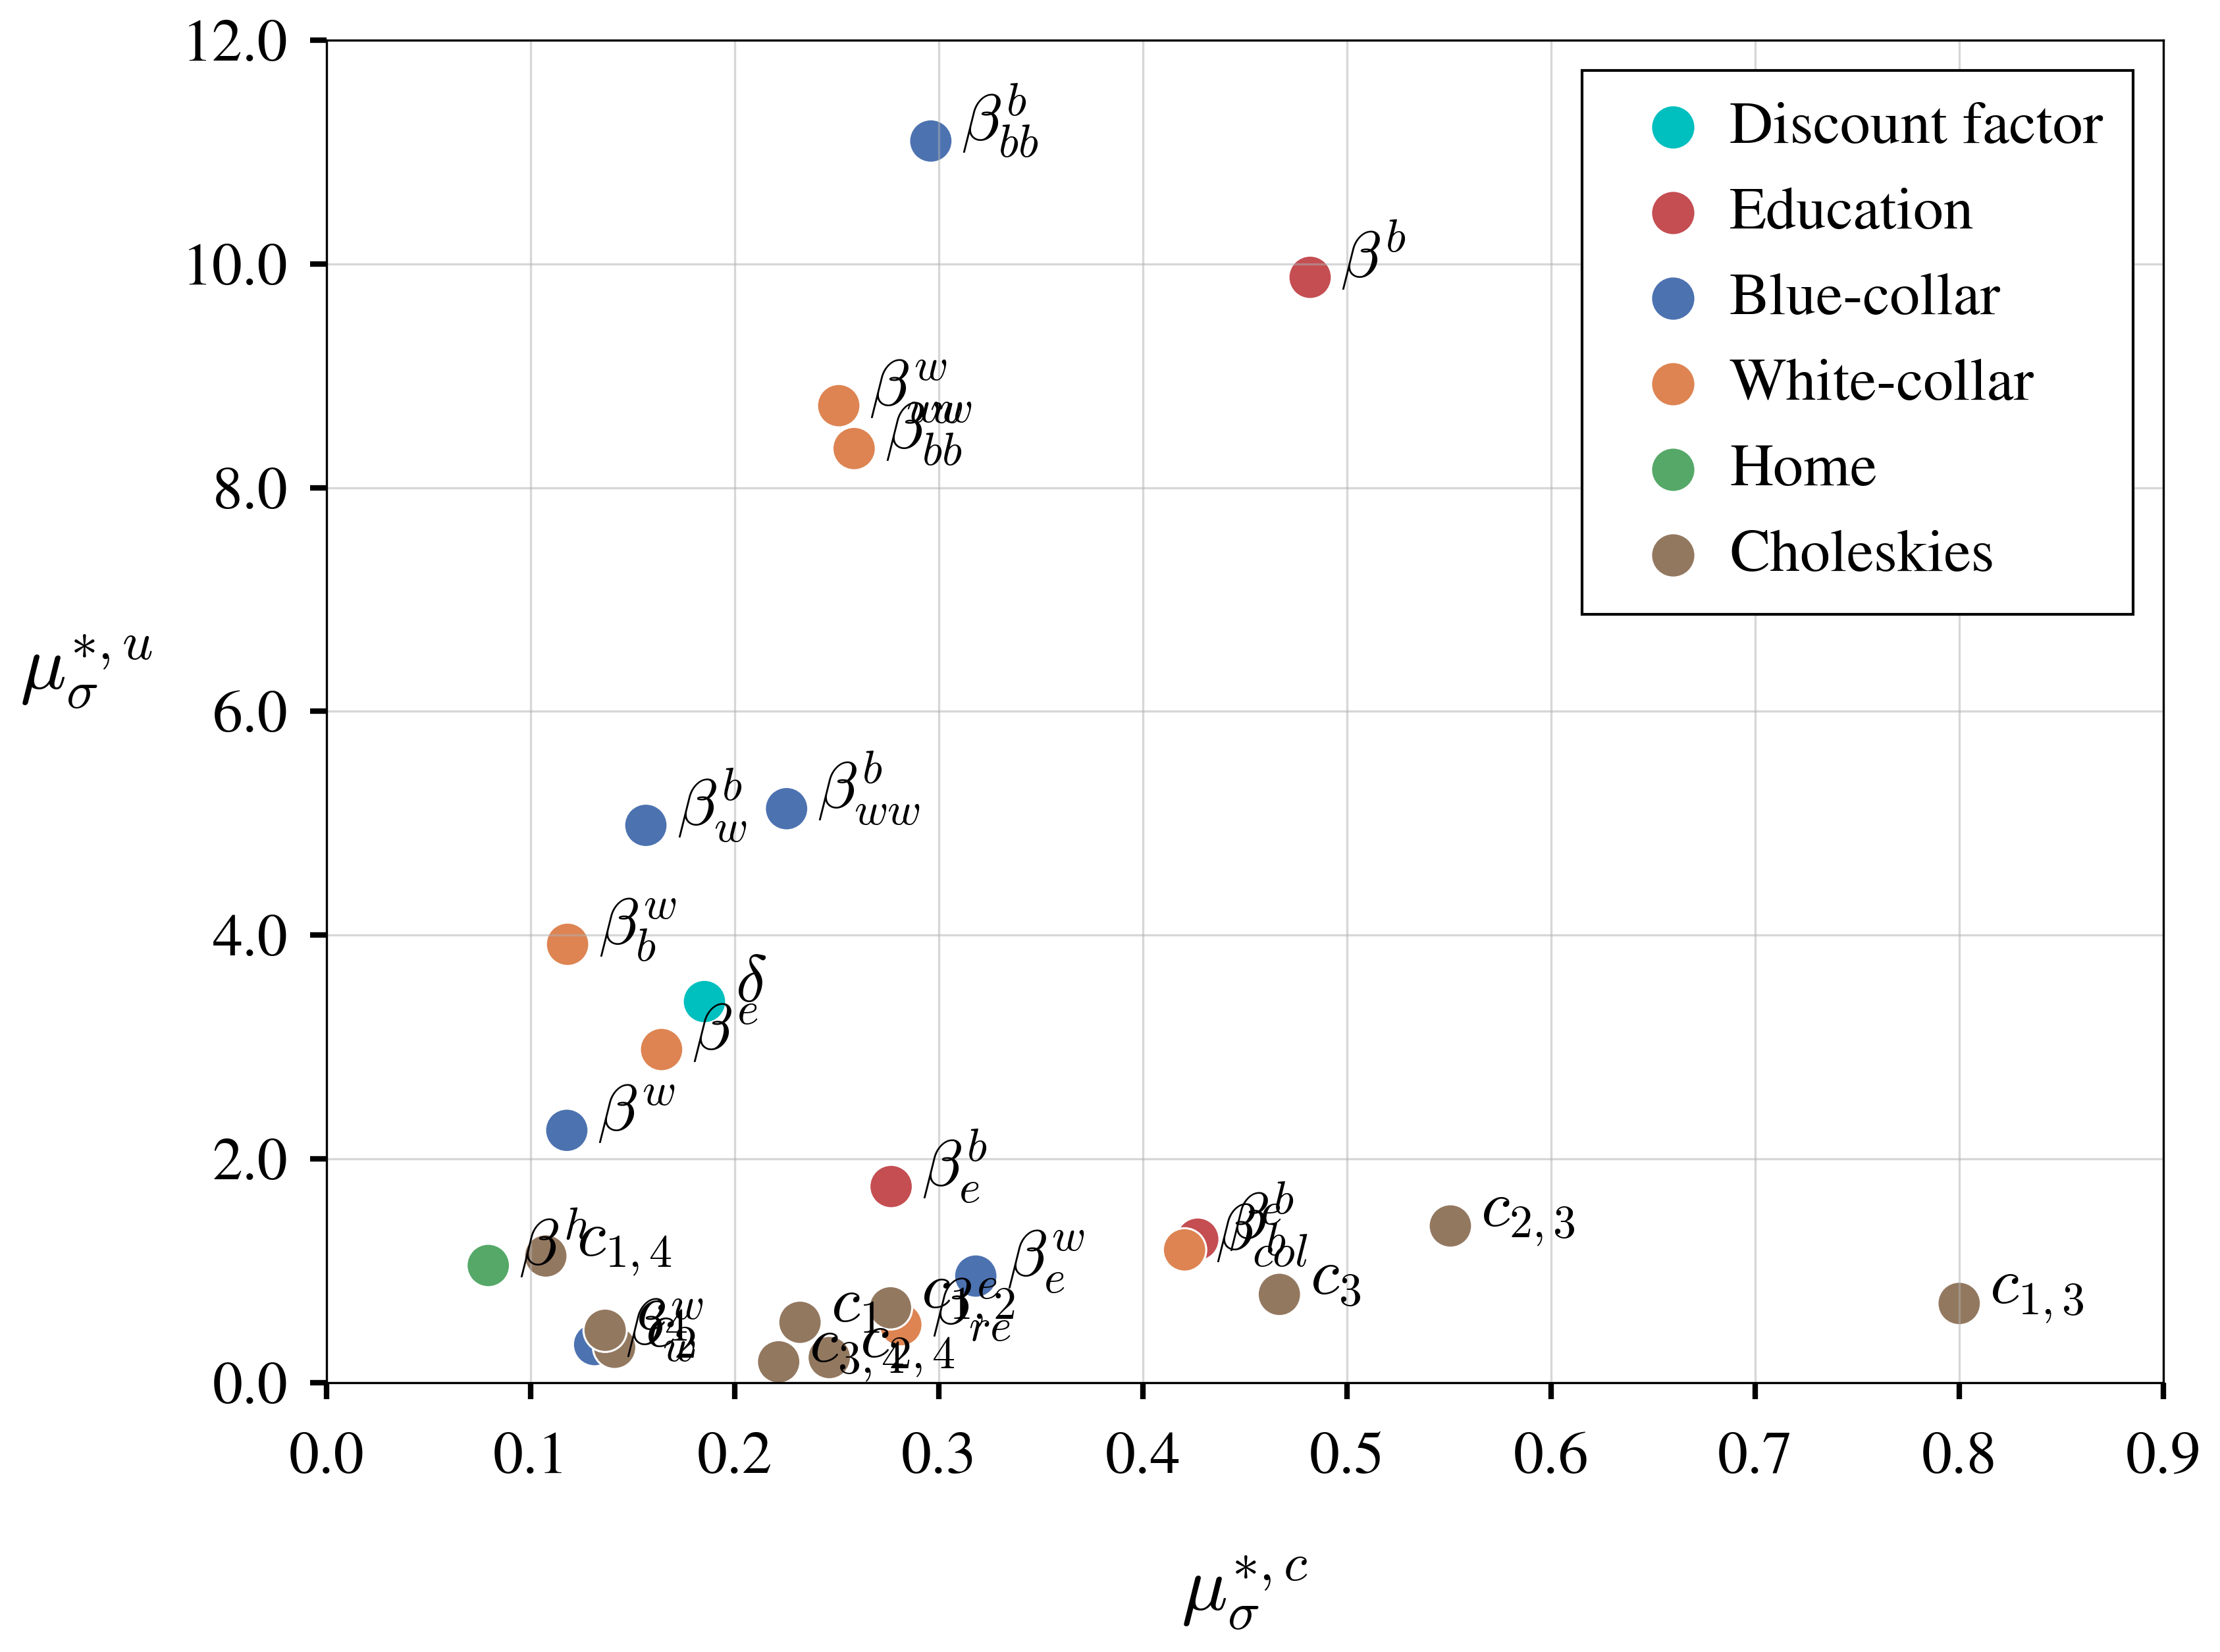
\includegraphics[scale=0.52]{../../../scrypy/figures/scatter_rad}
	\label{fig:rad}
\end{figure}


\newpage
\bibliography{../../bibliography/literature}

\end{document}